\subsection{Allimentations et masses électriques}
\label{subsec:alimentation}

Les systèmes de séquenceurs, d'allumage de l'inflamateur et de l'expérience générale (APEX et caméras) sont fortement isolés les
uns des autres, notamment au niveau de leurs alimentations électriques. En effet, chaque système dispose de son propre circuit
d'alimentation, de ces propres batteries et donc de ces propres masses électriques, ce qui permet d'assurer une meilleure
fiabilité et sécurité du système global: une défaillance ou un court-circuit dans un système n'affectera pas les autres systèmes.
De plus, cela permet de mieux gérer les consommations électriques de chaque système, en adaptant les capacités des batteries et
les circuits d'alimentation en fonction des besoins spécifiques de chaque système.\\

\begin{minipage}{0.5\textwidth}
Les principales batteries utilisées pour alimenter les différents systèmes de la fusée sont des batteries Li-Ion de 3.7V et
2.6Ah, comme celle présentée à la figure \ref{fig:batterie_RS}. Ces batteries sont choisies pour leur bonne densité énergétique,
leur fiabilité et la présence d'un circuit de protection intégré contre les surcharges, les décharges profondes et les
courts-circuits, ce qui est essentiel pour assurer la sécurité du système électronique de la fusée.\\
\end{minipage}
\hfill
\begin{minipage}{0.4\textwidth}
    \centering
    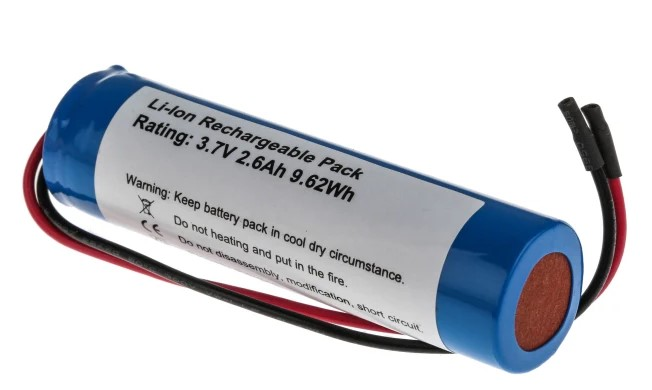
\includegraphics[width=\textwidth]{figures/batterie_RS.jpg}
    \captionof{figure}{Batterie Li-Ion 18650-26H}
    \label{fig:batterie_RS}
\end{minipage}

Dans chaque étage de la fusée, on trouve:
\begin{itemize}
    \item \textbf{\texttt{SEQUENCEUR}} : 2 batteries 18650-26H en bloc 1P2S (1 parallèle de 2 batteries en série) pour une
    tension totale de 7.4V et une capacité de 2.6Ah. Cette tension a été choisie pour coupler au choix de nos servomoteurs.
    \item \textbf{\texttt{EXPERIENCE}} : 2 batteries 18650-26H en bloc 2P1S (2 parallèles de 1 batterie en série) pour une
    tension totale de 3.7V et une capacité de 5.2Ah. Cette configuration a été choisie pour assurer une capacité suffisante pour
    alimenter l'ensemble des capteurs et des caméras embarquées pendant toute la durée de la mission, tout en maintenant une
    tension compatible avec les composants électroniques utilisés.\\ 
\end{itemize}

Pour ce qui est de l'alimentation du circuit d'allumage de la ligne de mise à feu du moteur du deuxième étage, elle est assurée
par une petite batterie Li-Po plate de 3.7V et 500mAh. Cette dernière a été choisi essentiellement pour son format compact et sa
capacité suffisante pour assurer la mise à feu du moteur du deuxième étage, qui ne nécessite pas une grande quantité d'énergie,
tout en permettant de réduire le poids et l'encombrement du système d'allumage.

\begin{figure}[h!]
    \centering
    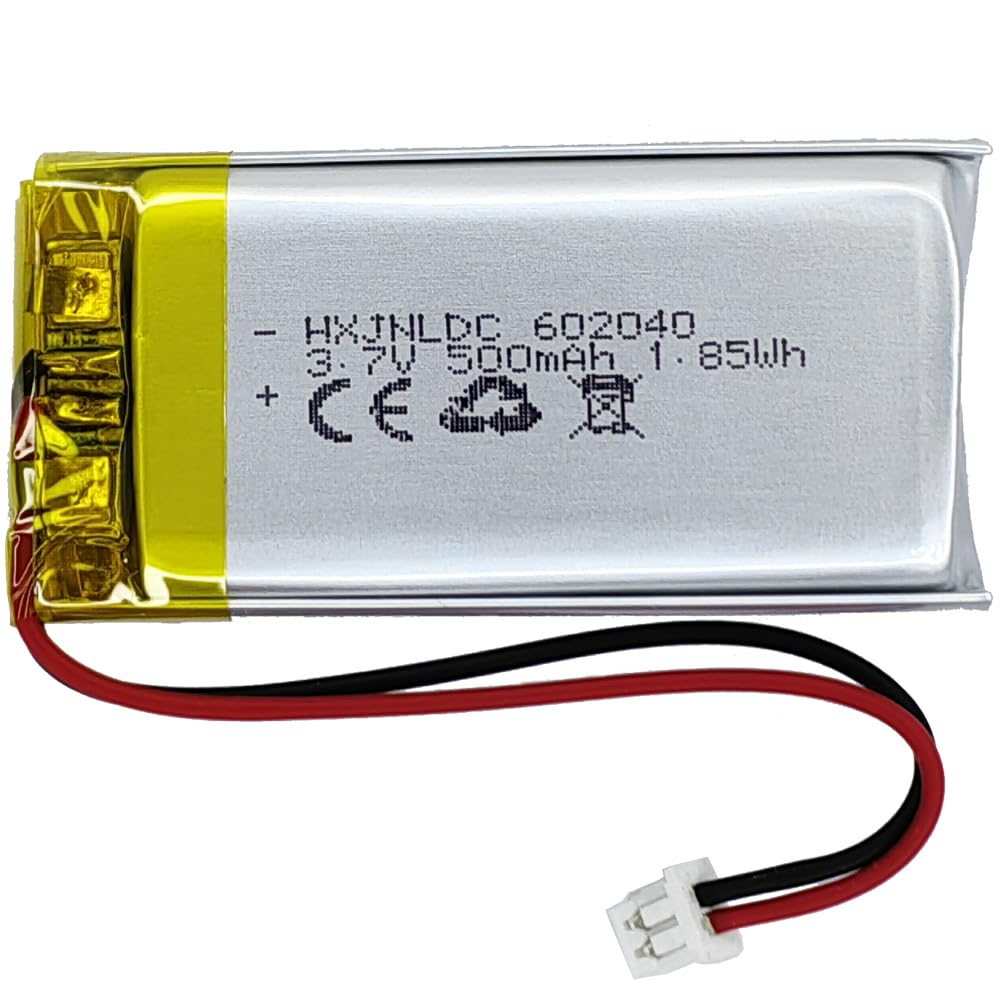
\includegraphics[width=0.5\textwidth]{figures/LiPo500.jpg}
    \caption{Batterie Li-Po plate}
    \label{fig:batterie_LiPo}
\end{figure}
